% Simulation Load -- Team Hallucinators, IML WS 26/27, Exercise 1
% LaTeX (Beamer) version of presentation/slides.html.
% Build:  uv run python scripts/make_latex_figures.py   (plots in figures/)
%         cd presentation/latex && tectonic slides.tex
\documentclass[aspectratio=169,11pt]{beamer}
\usetheme{Madrid}                      % blue title bar + three-part footline
\usepackage[utf8]{inputenc}
\usepackage{tikz}
\usetikzlibrary{positioning}
\setbeamertemplate{navigation symbols}{} % no navigation icons

% colours of the HTML deck
\definecolor{mblue}{HTML}{3333B2}
\definecolor{mgreen}{HTML}{2E8B57}
\definecolor{mred}{HTML}{C62828}
\definecolor{mlight}{HTML}{E6E6F6}
\definecolor{mredlight}{HTML}{F8E1E0}
\definecolor{mgrey}{HTML}{8F8FA8}

\title{Simulation Load}
\subtitle{How many steps to trace one prediction?}
\author[Team Hallucinators]{Kevin Antony \and Arsha Fahima Tajdeen \and Diya Panikkassery Sudheer Kumar\\[2pt]
  \small\textcolor{mblue}{\textbf{Team Hallucinators}}}
\institute[]{Interpretable Machine Learning WS 26/27 \textperiodcentered{} Exercise 1}
\date{}

% complete binary tree: #1 x of root, #2 y of root, #3 depth, #4 width, #5 height, #6 colour
\newcommand{\bintree}[6]{%
  \foreach \l in {1,...,#3}{%
    \pgfmathtruncatemacro\n{2^\l-1}%
    \foreach \i in {0,...,\n}{%
      \pgfmathsetmacro\xx{#1-#4/2+#4*(\i+0.5)/2^\l}%
      \pgfmathsetmacro\yy{#2-#5*\l/#3}%
      \pgfmathsetmacro\px{#1-#4/2+#4*(floor(\i/2)+0.5)/2^(\l-1)}%
      \pgfmathsetmacro\py{#2-#5*(\l-1)/#3}%
      \draw[#6, thick] (\px,\py) -- (\xx,\yy);}}%
  \foreach \l in {0,...,#3}{%
    \pgfmathtruncatemacro\n{2^\l-1}%
    \foreach \i in {0,...,\n}{%
      \pgfmathsetmacro\xx{#1-#4/2+#4*(\i+0.5)/2^\l}%
      \pgfmathsetmacro\yy{#2-#5*\l/#3}%
      \filldraw[fill=white, draw=#6, thick] (\xx,\yy) circle (2.2pt);}}}

\begin{document}

% ---------------------------------------------------------------- 1 title
\begin{frame}[plain]
  \titlepage
\end{frame}

% ---------------------------------------------------------------- 2 question
\begin{frame}{When does a tree model stop being interpretable?}
  \centering
  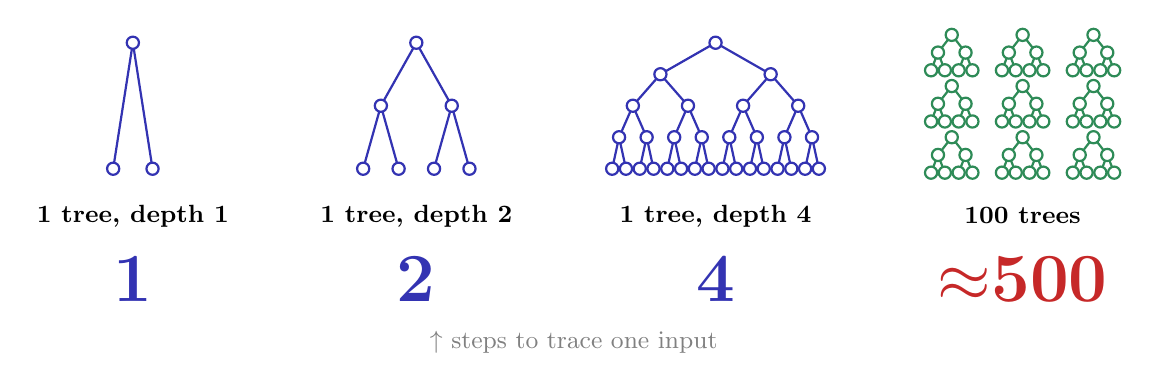
\begin{tikzpicture}
    \bintree{0}{3}{1}{1.0}{1.6}{mblue}
    \bintree{3.6}{3}{2}{1.8}{1.6}{mblue}
    \bintree{7.4}{3}{4}{2.8}{1.6}{mblue}
    \foreach \r in {0,1,2}{\foreach \c in {0,1,2}{\bintree{10.4+\c*0.9}{3.1-\r*0.65}{2}{0.7}{0.45}{mgreen}}}
    \foreach \x/\name/\n/\col in {0/{1 tree, depth 1}/1/mblue, 3.6/{1 tree, depth 2}/2/mblue,
                                  7.4/{1 tree, depth 4}/4/mblue, 11.3/{100 trees}/{$\approx$500}/mred}{
      \node[font=\small\bfseries] at (\x,0.8) {\name};
      \node[font=\Huge\bfseries, text=\col] at (\x,0) {\n};}
    \node[font=\small, text=gray] at (5.6,-0.8) {$\uparrow$ steps to trace one input};
  \end{tikzpicture}
\end{frame}

% ---------------------------------------------------------------- 3 idea
\begin{frame}{Our idea: count the steps}
  \begin{columns}[c]
    \begin{column}{0.66\textwidth}
      \centering
      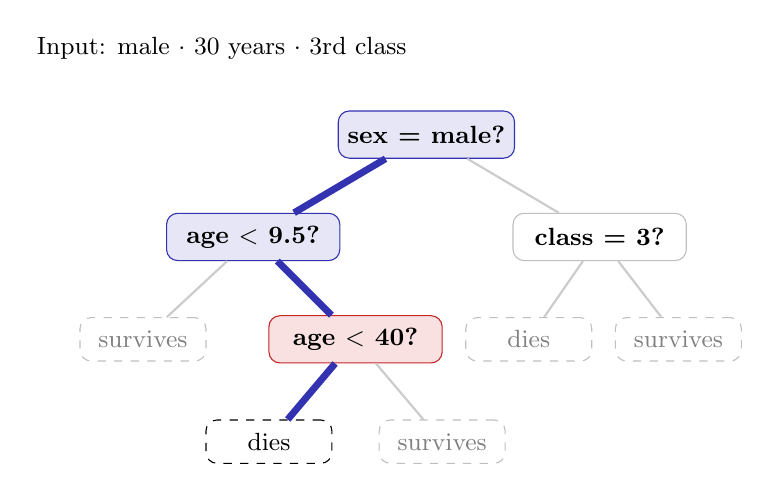
\begin{tikzpicture}[q/.style={draw=gray!50, rounded corners, minimum width=2.2cm, minimum height=0.6cm, font=\small\bfseries},
                          leaf/.style={draw=gray!50, dashed, rounded corners, minimum width=1.6cm, minimum height=0.55cm, font=\small, text=gray},
                          on/.style={draw=mblue, fill=mlight}, path/.style={mblue, line width=2.5pt}]
        \node[font=\small] (in) at (-2.6,1.1) {Input: male $\cdot$ 30 years $\cdot$ 3rd class};
        \node[q, on] (n0) at (0,0) {sex = male?};
        \node[q, on] (n1) at (-2.2,-1.3) {age $<$ 9.5?};
        \node[q] (n2) at (2.2,-1.3) {class = 3?};
        \node[leaf] (l1) at (-3.6,-2.6) {survives};
        \node[q, draw=mred, fill=mredlight] (n3) at (-0.9,-2.6) {age $<$ 40?};
        \node[leaf] (l2) at (1.3,-2.6) {dies};
        \node[leaf] (l3) at (3.2,-2.6) {survives};
        \node[leaf, draw=black, text=black] (l4) at (-2.0,-3.9) {dies};
        \node[leaf] (l5) at (0.2,-3.9) {survives};
        \draw[gray!40, thick] (n0) -- (n2) (n1) -- (l1) (n2) -- (l2) (n2) -- (l3) (n3) -- (l5);
        \draw[path] (n0) -- (n1); \draw[path] (n1) -- (n3); \draw[path] (n3) -- (l4);
      \end{tikzpicture}
    \end{column}
    \begin{column}{0.3\textwidth}
      \large\ttfamily
      +1 \ sex\\[4pt]
      +1 \ age\\[4pt]
      \textcolor{mred}{+½ age} {\normalsize\textcolor{gray}{again}}\\[2pt]
      \rule{3.2cm}{1pt}\\[2pt]
      {\Huge\textbf{\textcolor{mblue}{2.5}}} \textrm{\textbf{steps}}
    \end{column}
  \end{columns}
\end{frame}

% ---------------------------------------------------------------- 4 metric
\begin{frame}{The metric}
  \centering\vspace{0.4cm}
  {\Large\bfseries
  load $=$ $\displaystyle\sum_{\text{trees}}$ \Big(
  $\underbrace{\textcolor{mblue}{\text{new features}}}_{\substack{\text{\normalsize\textcolor{mblue}{look up}}\\\text{\normalsize\textcolor{mblue}{+ compare}}}}$
  $+$
  $\underbrace{\textcolor{mred}{\tfrac12 \cdot \text{repeats}}}_{\text{\normalsize\textcolor{mred}{compare only}}}$
  \Big) $+$
  $\underbrace{\textcolor{mgreen}{(\text{trees} - 1)}}_{\text{\normalsize\textcolor{mgreen}{combine the trees}}}$}

  \vspace{0.4cm}
  {\textcolor{gray}{averaged over all inputs in the data}}

  \vspace{0.6cm}
  \begin{minipage}{0.6\textwidth}
    \begin{alertblock}{Threshold}
      \centering {\Huge\bfseries load $\le$ 7} \quad \textcolor{gray}{working memory: 7 $\pm$ 2 items}
    \end{alertblock}
  \end{minipage}
\end{frame}

% ---------------------------------------------------------------- 5 leaves vs load
\begin{frame}{Same size, very different effort}
  \centering
  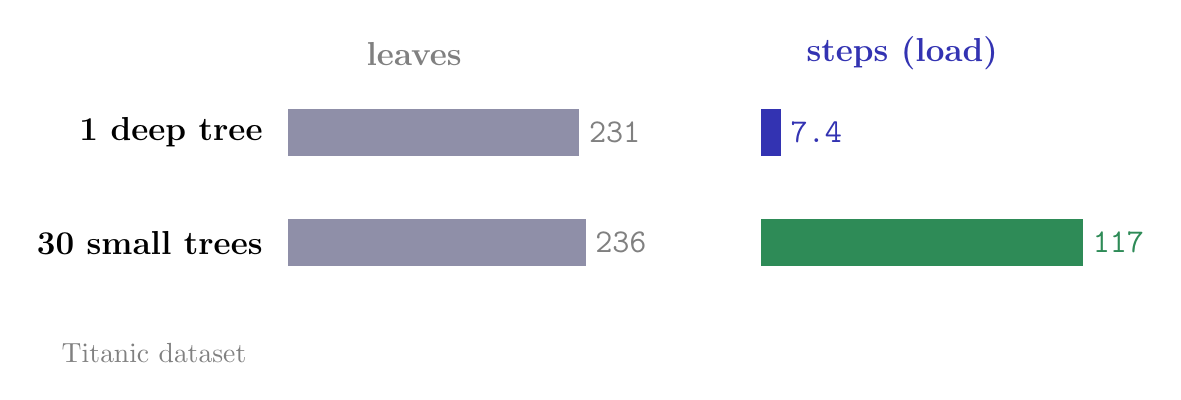
\begin{tikzpicture}[x=1cm, y=1cm, lab/.style={anchor=east, font=\large\bfseries}, val/.style={anchor=west, font=\large\ttfamily\bfseries}]
    \node[font=\large\bfseries, text=gray] at (4.6,2.2) {leaves};
    \node[font=\large\bfseries, text=mblue] at (10.8,2.2) {steps (load)};
    % row 1: one deep tree
    \node[lab] at (2.8,1.2) {1 deep tree};
    \fill[mgrey] (3,0.9) rectangle ++(231*0.016,0.6);  \node[val, text=gray] at (3+231*0.016,1.2) {231};
    \fill[mblue] (9,0.9) rectangle ++(7.4*0.035,0.6);  \node[val, text=mblue] at (9+7.4*0.035,1.2) {7.4};
    % row 2: forest of 30 small trees
    \node[lab] at (2.8,-0.2) {30 small trees};
    \fill[mgrey] (3,-0.5) rectangle ++(236*0.016,0.6); \node[val, text=gray] at (3+236*0.016,-0.2) {236};
    \fill[mgreen] (9,-0.5) rectangle ++(117*0.035,0.6); \node[val, text=mgreen] at (9+117*0.035,-0.2) {117};
    \node[text=gray, anchor=west] at (0,-1.6) {Titanic dataset};
  \end{tikzpicture}
\end{frame}

% ---------------------------------------------------------------- 6 experiment
\begin{frame}{Experiment}
  \centering
  \begin{columns}[t]
    \begin{column}{0.3\textwidth}\centering
      {\fontsize{48}{50}\selectfont\bfseries\textcolor{mblue}{6}}\\[4pt] {\large datasets}\\[6pt]
      \small\textcolor{gray}{banknote $\cdot$ breast cancer $\cdot$ titanic $\cdot$ diabetes $\cdot$ credit-g $\cdot$ phoneme}
    \end{column}
    \begin{column}{0.3\textwidth}\centering
      {\fontsize{48}{50}\selectfont\bfseries\textcolor{mblue}{65}}\\[4pt] {\large models}\\[6pt]
      \small\textbf{\textcolor{mblue}{1 tree}} $\cdot$ \textbf{\textcolor{mgreen}{forest}} $\cdot$ \textbf{\textcolor{mred}{boosting}}\\
      \textcolor{gray}{1 -- 100 trees}
    \end{column}
    \begin{column}{0.3\textwidth}\centering
      {\fontsize{48}{50}\selectfont\bfseries\textcolor{mblue}{3}}\\[4pt] {\large train/test splits}
    \end{column}
  \end{columns}
\end{frame}

% ---------------------------------------------------------------- 7 accuracy vs load
\begin{frame}{Accuracy vs.\ load}
  \centering
  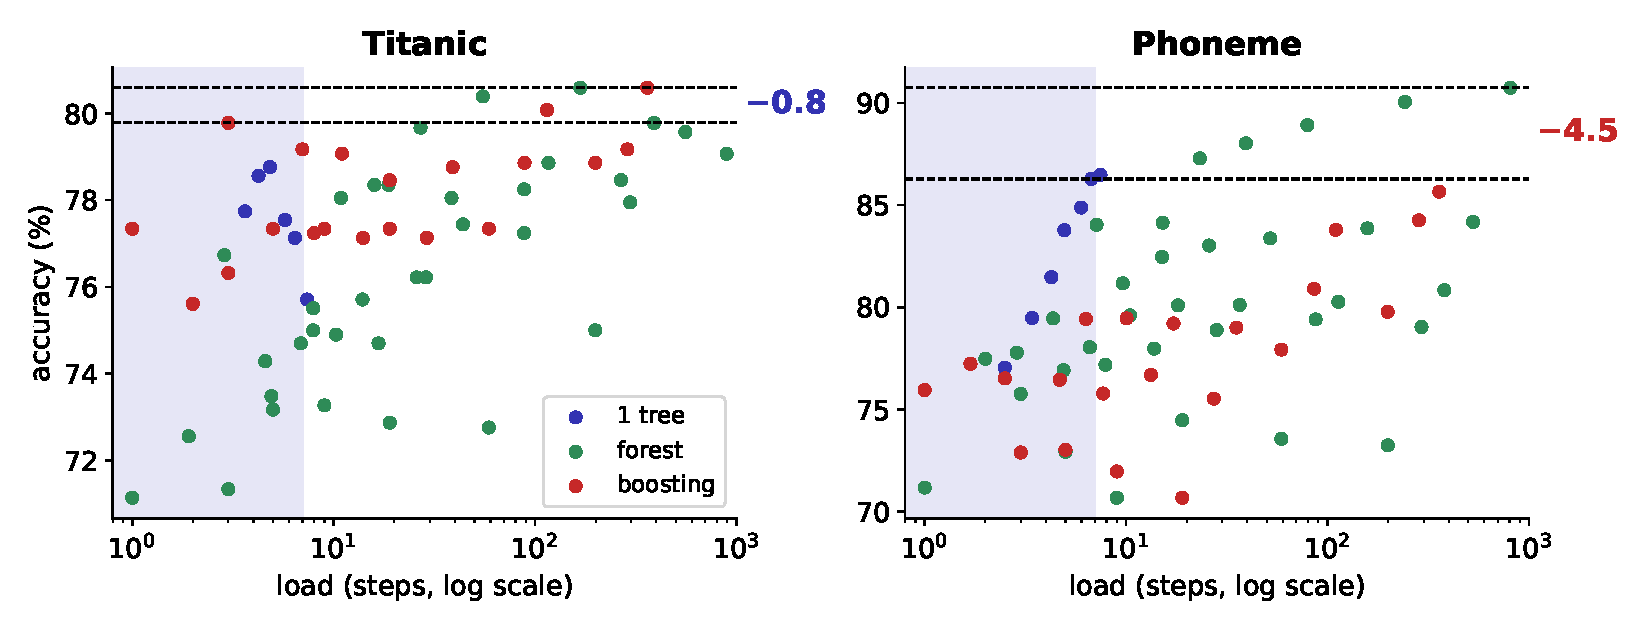
\includegraphics[width=\textwidth]{figures/scatter.pdf}\\
  \small\textcolor{gray}{shaded: interpretable (load $\le$ 7) \quad dashed: best model overall vs.\ best interpretable model}
\end{frame}

% ---------------------------------------------------------------- 8 price
\begin{frame}{Price of staying interpretable}
  \centering
  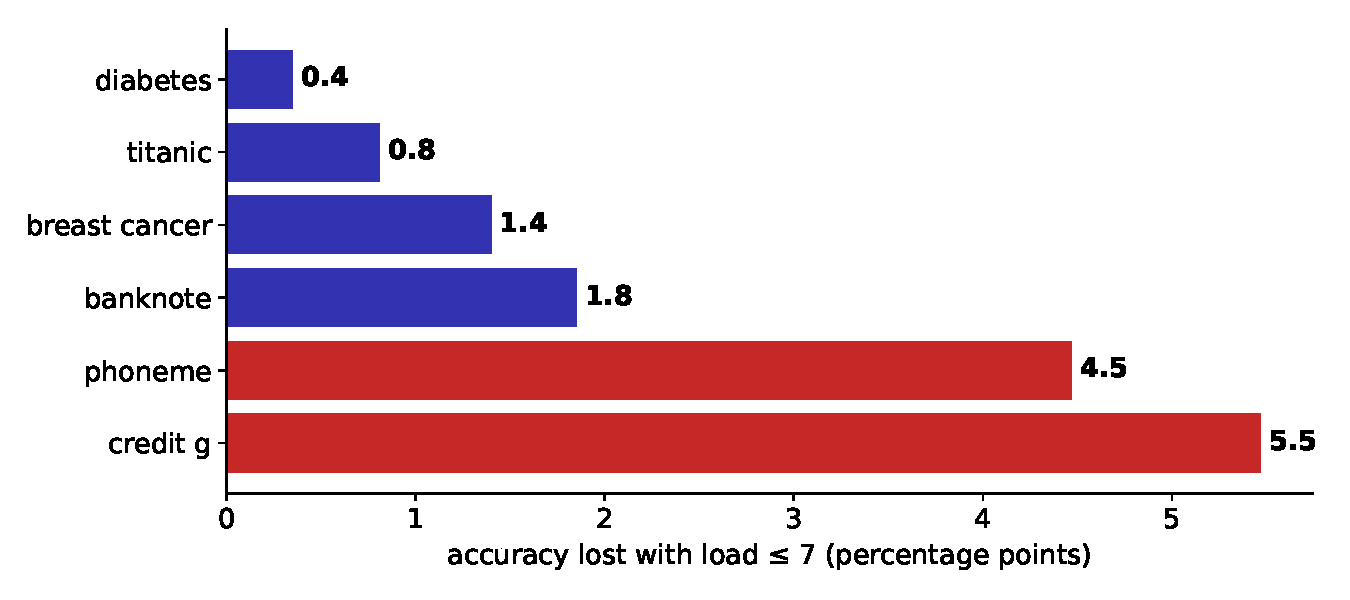
\includegraphics[width=0.85\textwidth]{figures/price.pdf}
\end{frame}

% ---------------------------------------------------------------- 9 threshold
\begin{frame}{Ensembles lose it after 2--3 trees}
  \centering
  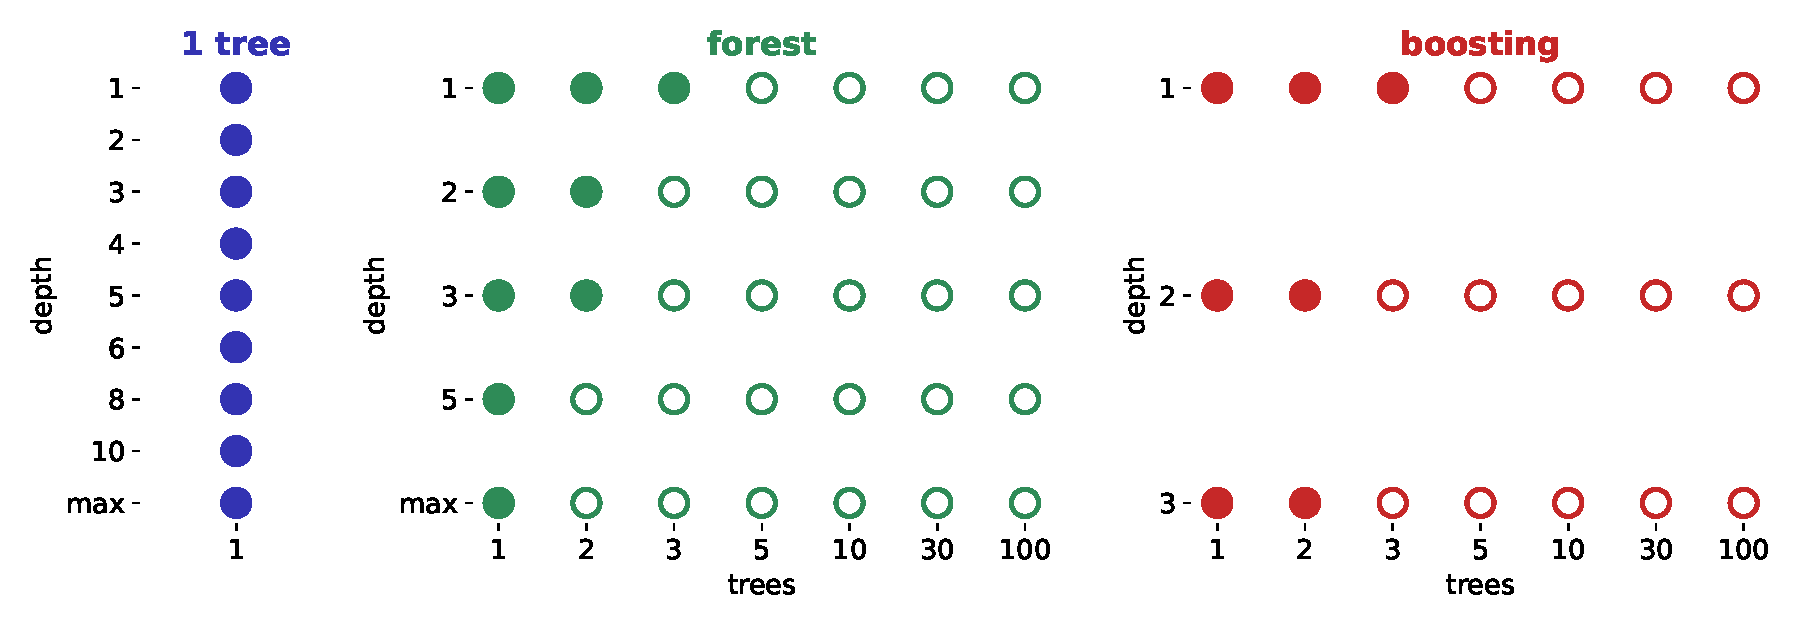
\includegraphics[width=\textwidth]{figures/threshold.pdf}\\
  \small\textcolor{gray}{filled: median load $\le$ 7 \quad hollow: load $>$ 7 \quad (median over 6 datasets)}
\end{frame}

% ---------------------------------------------------------------- 10 task 2 correlations
\begin{frame}{Task 2: what makes a dataset expensive?}
  \centering
  \small\textcolor{gray}{32 OpenML datasets $\cdot$ correlation with \textbf{accuracy lost at load $\le$ 7}}\\
  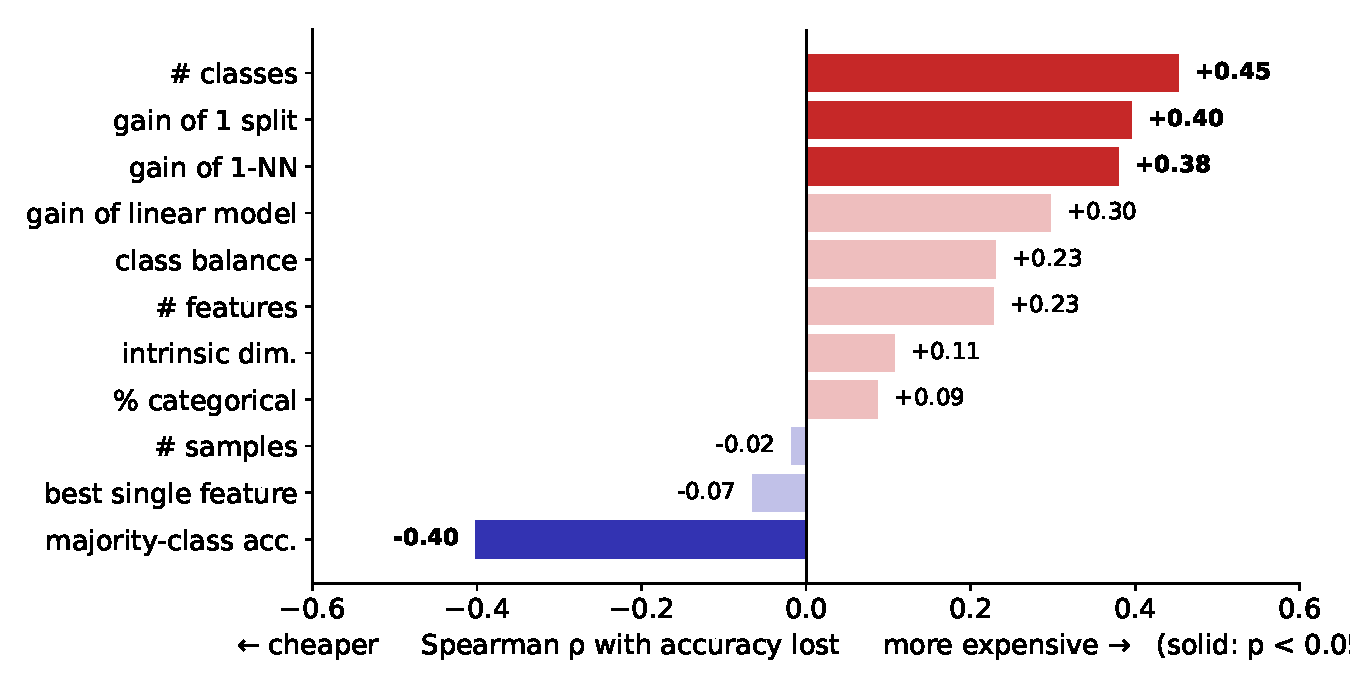
\includegraphics[width=0.85\textwidth]{figures/task2_corr.pdf}
\end{frame}

% ---------------------------------------------------------------- 11 task 2 scatter
\begin{frame}{More classes cost more, imbalance is cheap}
  \centering
  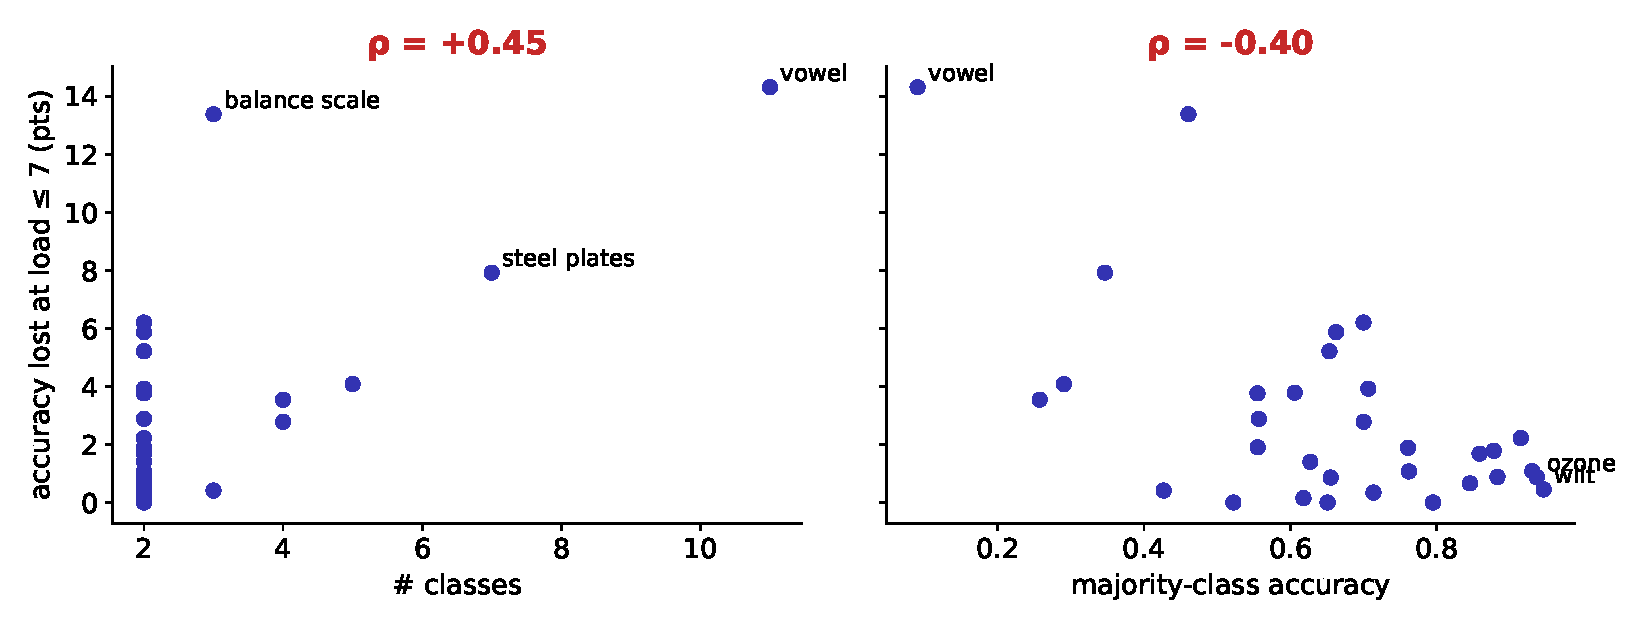
\includegraphics[width=\textwidth]{figures/task2_scatter.pdf}
\end{frame}

% ---------------------------------------------------------------- 12 meta tree
\begin{frame}{Can we tell before training?}
  \centering
  \begin{tikzpicture}[box/.style={draw=gray!60, rounded corners, minimum height=0.7cm, font=\small\bfseries, align=center},
                      edge/.style={gray, thick}]
    \node[box, minimum width=6cm] (r) at (0,0) {best single feature: $|$corr$|$ $\le$ 0.26 ?};
    \node[box, draw=mblue, fill=mlight, minimum width=3.4cm] (a) at (-3.6,-1.8) {simple tree enough\\\textcolor{mblue}{\ttfamily 4 / 4 datasets}};
    \node[box, minimum width=3.4cm] (b) at (3,-1.8) {$|$corr$|$ $\le$ 0.39 ?};
    \node[box, draw=mred, fill=mredlight, minimum width=3.4cm] (c) at (1,-3.6) {complex model needed\\\textcolor{mred}{\ttfamily 12 / 12 datasets}};
    \node[box, minimum width=3cm] (d) at (5,-3.6) {mixed\\\textcolor{gray}{\ttfamily 7 of 16 simple}};
    \draw[edge] (r) -- node[above left, font=\small, text=gray] {yes} (a);
    \draw[edge] (r) -- node[above right, font=\small, text=gray] {no} (b);
    \draw[edge] (b) -- (c); \draw[edge] (b) -- (d);
    \node[anchor=north west] at (-6.2,-2.9) {\begin{minipage}{4.2cm}
      \begin{block}{Leave-one-out accuracy}
        {\LARGE\bfseries 75\%} \small vs.\ 66\% guessing
      \end{block}\end{minipage}};
  \end{tikzpicture}
\end{frame}

% ---------------------------------------------------------------- 13 limits
\begin{frame}{Limits}
  \Large
  \begin{itemize}\setlength\itemsep{14pt}
    \item No user study: 1, ½ and 7 are assumptions
    \item One prediction, not the whole model
    \item Ignores what the features mean
    \item Task 2: 32 datasets, 44 tests $\rightarrow$ hints, not proof
  \end{itemize}
\end{frame}

% ---------------------------------------------------------------- 14 AI
\begin{frame}{How we used AI}
  \Large
  \begin{block}{Claude Code (Claude Opus 5.5)}
    Code, experiments
  \end{block}
  \vspace{0.5cm}
  \begin{alertblock}{Checked by us}
    Read the code, re-ran everything, verified the numbers
  \end{alertblock}
\end{frame}

% ---------------------------------------------------------------- 15 takeaway
\begin{frame}{Takeaway}
  \begin{block}{Interpretable}
    \centering\vspace{4pt}{\LARGE\bfseries a prediction can be traced in $\le$ 7 steps}\vspace{4pt}
  \end{block}
  \vspace{0.5cm}
  \begin{columns}[t]
    \begin{column}{0.23\textwidth}\begin{block}{1 tree}\centering\large\bfseries $\le$ 7 \checkmark\end{block}\end{column}
    \begin{column}{0.23\textwidth}\begin{alertblock}{Ensembles}\centering\large\bfseries $>$ 7 after 2--3 trees\end{alertblock}\end{column}
    \begin{column}{0.23\textwidth}\begin{block}{Accuracy cost}\centering\large\bfseries 0.4 -- 5.5 pts\end{block}\end{column}
    \begin{column}{0.23\textwidth}\begin{block}{Costly datasets}\centering\large\bfseries many classes, balanced\end{block}\end{column}
  \end{columns}
\end{frame}

\end{document}
